\section{MLOps}\label{sec:mlops}

In this section we will try to describe key aspect of MLOps as can be found in today's literature.

\subsection{Description}\label{subsec:description}
MLOps or Machine Learning Operations is the organisation and automation of Machine learning development workflow and operations.
It's an extension of DevOps practices adapted to machine learning model development and data operations\cite{Kreuzberger2022MachineLO}.
MLOps is almost never taken alone and DataOps is an integrated part of the full MLOps lifecycle.

MLOps with clearly defined workflow and infrastructure can provide transparency and accountability to Upper Management and Business.\cite{treveil2020introducing}(p.11)

\begin{figure}[!htbp]
    \caption{MLOps lifecycle\cite{mlops-definition-tools-and-challenge}}
    \centering
    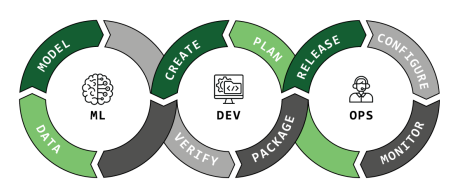
\includegraphics[scale=0.5]{images/ml-dev-ops}
    \label{fig:ml-dev-ops}
\end{figure}

MLOps is essential for data teams and organisations, as it involves a complex integration of technologies, processes, and people, requiring ongoing discipline and time to implement effectively.
It is not a one-time task but a continuous effort to ensure successful machine learning operations.\cite{treveil2020introducing}(p.38)

A survey in 2021\cite{DBLP:journals/corr/abs-2103-08942} already show that Machine Learning development is evolving towards team-based development.
They also show that in a result the adoption of DevOps practices is increasing and the required skills in infrastructure and deployment are evolving.

In this regard, they also identified the following obstacles among others\cite{DBLP:journals/corr/abs-2103-08942}:
    \begin{itemize}
        \item Accessibility of data
        \item Building training pipelines
        \item Deployment and target environment (on-premise, cloud)
        \item Tracking and comparing training
        \item Collaborating on projects
        \item Lack of guidelines
    \end{itemize}

Since then, we will see that some of those difficulties have been tackled, tools exist and are currently reviewed in the literature.

In 2025, in their systematic literature review\cite{10855428}, they still consider MLOps as an emerging field.
But they admit, publications are still limited.
Variations in defining and grouping steps for creating and maintaining models arise from differing interpretations,
model architectures, and usage methods, leading to diverse implementation approaches.

\subsection{Challenges}\label{subsec:challenges}

Adopting MLOps presents challenges, as highlighted by\cite{Kreuzberger2022MachineLO}, which categorizes them into organizational,
ML system, and operational issues.
Organizational challenges include shifting to a product-oriented mindset, addressing skill shortages,
and fostering multidisciplinary teamwork, while ML system challenges focus on scalability and fluctuating demand,
and operational challenges emphasize automation, governance, and reproducibility.
These challenges are closely tied to the deployment stage in ML workflows, which involves critical steps like data management,
model training, and deployment, each accompanied by issues such as data dispersion, resource constraints, and also ethical concerns\cite{10.1145/3533378}.
All together, these challenges and considerations mark the complexity of implementing MLOps effectively.

In their publication, a Microsoft team\cite{8804457} outlined challenges for MLOps implementation, including Data Availability, Collection, Cleaning, and Management,
Education and Training, and Hardware Resources.
They also highlighted the need for End-to-end Pipeline Support, Model Evolution, Evaluation, and Deployment, and effective Collaboration and Working Culture.
Additionally, challenges like Integrating AI into Larger Systems, AI Tools, and Scale were emphasized,
along with the importance of Guidance and Mentoring for skill development.
These challenges highlight the multifaceted nature of MLOps, requiring both technical and organizational solutions.

\subsection{Roles in MLOps}\label{subsec:actors}

Machine learning development has evolved into a collaborative, team-based process involving diverse roles.
Each role, from business experts to technical architects, contributes to the lifecycle of Machine Learning models.
Their responsibilities include ensuring model maintenance, optimization, trust in deployment,
and mitigating business risks\cite{treveil2020introducing}(p.22).

The data scientist is often considered the central role in this process.
However, within the context of MLOps, the literature identifies several key roles that
collaborate to support the development and deployment of machine learning models.
These roles include\cite{treveil2020introducing}(p.14):
Subject-Matter Experts, Data Scientists, Data Engineers, DevOps engineers, Software engineers, Model Risk Managers, Machine Learning architects.
Additional literature further refines these roles, proposing the following\cite{Kreuzberger2022MachineLO}:

\begin{itemize}
    \item Business Stakeholder
    \item Solution Architect
    \item Data Scientist
    \item Data Engineer
    \item Software Engineer
    \item DevOps Engineer
    \item ML Engineer/MLOps Engineer
\end{itemize}

\textit{Each person—from the subject-matter-expert on the business side to the most
technical machine learning architect—plays a critical part in the maintenance of ML
models in production}\cite{treveil2020introducing}(p.22).

In figure\ref{fig:mlop-people}, they propose an example of those roles within an organization.
\begin{figure}[!htbp]
    \caption{Realistic picture of a machine learning model life cycle inside an average
    organisation today\cite{treveil2020introducing}(p.6)}
    \centering
    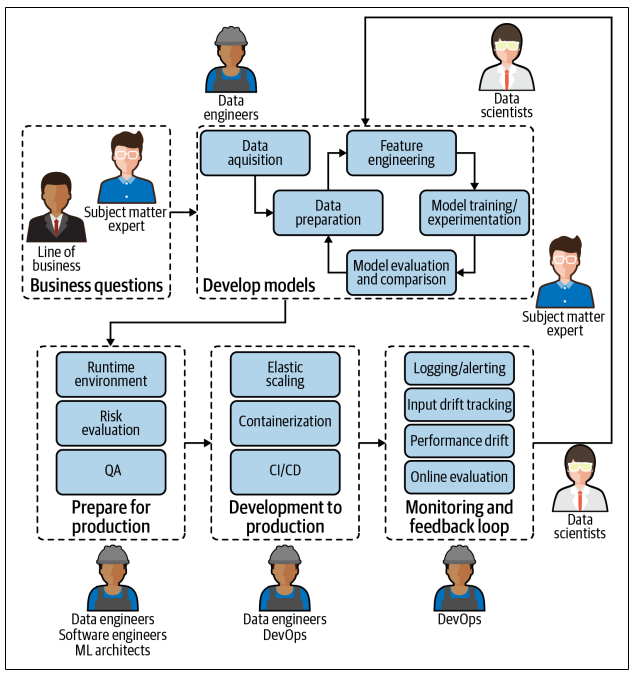
\includegraphics[scale=0.5]{images/mlops-people}
    \label{fig:mlop-people}
\end{figure}

\subsection{Workflow}\label{subsec:workflow}

In their review\cite{Kreuzberger2022MachineLO}, they extracted good practices and principles to implement a MLOps workflow:

\begin{itemize}
    \item CI/CD automation
    \item Workflow orchestration
    \item Reproducibility
    \item Versioning of data, code and model. (I would add versioning of pipelines)
    \item Collaboration
    \item Continuous ML training and evaluation
    \item ML metadata tracking
    \item Continuous Monitoring
    \item Feedback loops
\end{itemize}

As we explained earlier those principles shares a lot with actual DevOps practices with the addition of ML considerations
like training and metadata tracking.

In\cite{9792270} They propose a workflow that shares many aspect with other workflows like those found in\cite{treveil2020introducing,gift2021practical}

\begin{figure}[!htbp]
    \caption{Proposed workflow in\cite{9792270}}
    \centering
    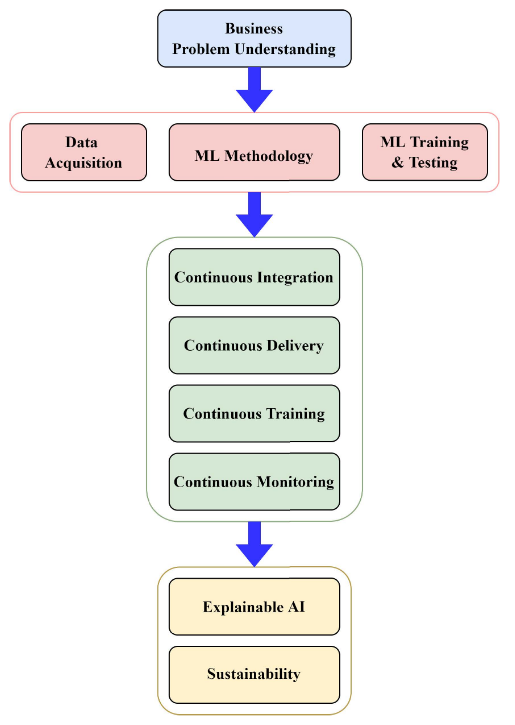
\includegraphics[scale=0.5]{images/taxo-workflow}
    \label{fig:taxo-workflow}
\end{figure}

\subsubsection{MLOps workflow methodology}
State-of-the-art MLOps component that should be used for any models\cite{BURGUENOROMERO2025107499}:
\begin{itemize}
    \item Model registry to release models.
    \item Pipeline orchestrator allows automation and reproducibility of MLOps workflows.
    \item Model serving platform to deploy models.
    \item Deployed model resources usually as REST/gRPC APIs
    \item Monitoring system as usual monitoring and feedback is mandatory
    \item Triggers when more automation comes into places it become mandatory to describe well-defined triggers for pipelines.
\end{itemize}

\subsubsection{Developing Models}
\begin{figure}[!htbp]
    \caption{Model development highlighted in the larger context of the ML project life
    cycle\cite{treveil2020introducing}(p.41)}
    \centering
    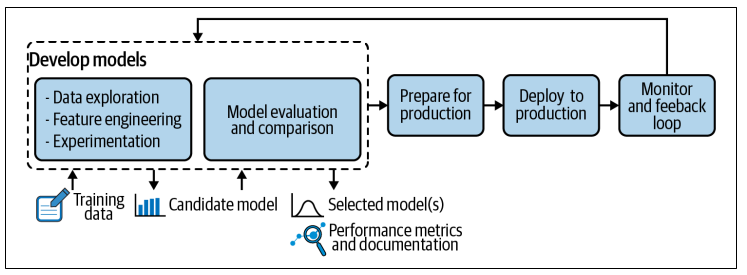
\includegraphics[scale=0.5]{images/developing-models-intro}
    \label{fig:developing-models-intro}
\end{figure}

\subsubsection{Training}

\subsubsection{Testing}
Beyond accuracy, factors like robustness, security, transparency, fairness, and safety are critical for building reliable and ethical AI\cite{10.1145/3555803}.

\subsubsection{Prepare for production}

\begin{figure}[!htbp]
    \caption{Preparing for production highlighted in the larger context of the ML project
    life cycle\cite{treveil2020introducing}(p.59)}
    \centering
    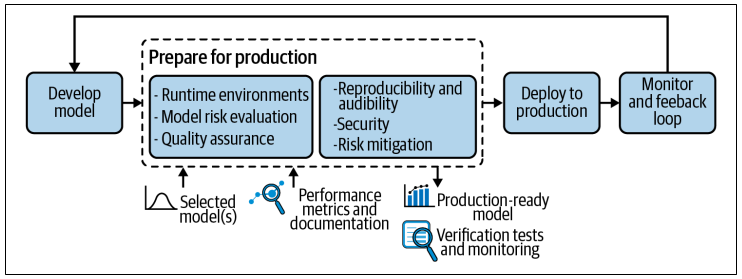
\includegraphics[scale=0.5]{images/prep-prod-intro}
    \label{fig:prep-prod-intro}
\end{figure}


\subsubsection{Deploy in production}

CI/CD (Continuous Integration/Continuous Deployment) principles, commonly used in traditional software engineering, are equally critical for machine learning systems and form a key part of MLOps strategies.
After developing a model, a data scientist should push code, metadata, and documentation to a central repository, triggering a CI/CD pipeline.
An example pipeline includes the following steps\cite{treveil2020introducing}(p.74).

\subsubsubsection{Develop the model:}
\begin{itemize}
    \item Create model artifacts
    \item Store artifacts in long-term storage
    \item Run basic checks
    \item Generate fairness and explainability reports
\end{itemize}
\subsubsubsection{Deploy to a Test Environment:}
\begin{itemize}
    \item Validate ML and computational performance
    \item Conduct manual validation
\end{itemize}
\subsubsubsection{Deploy to Production:}
\begin{itemize}
    \item Roll out the model incrementally (e.g., as a canary deployment)
    \item Fully deploy the model once validated
\end{itemize}

\begin{figure}[!htbp]
    \caption{Preparing for production highlighted in the larger context of the ML project
    life cycle\cite{treveil2020introducing}(p.73)}
    \centering
    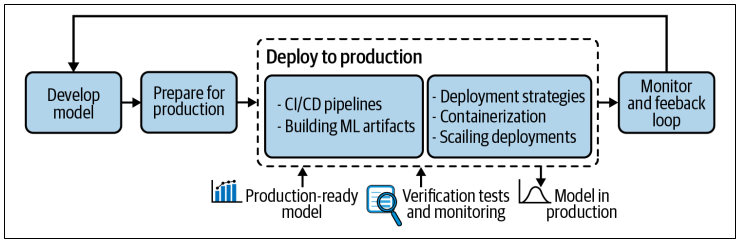
\includegraphics[scale=0.5]{images/deploy-prod}
    \label{fig:deploy-prod}
\end{figure}


\subsubsection{Monitor and FeedBack}

\begin{figure}[!htbp]
    \caption{Monitoring and feedback loop highlighted in the larger context of the ML
    project life cycle\cite{treveil2020introducing}(p.85)}
    \centering
    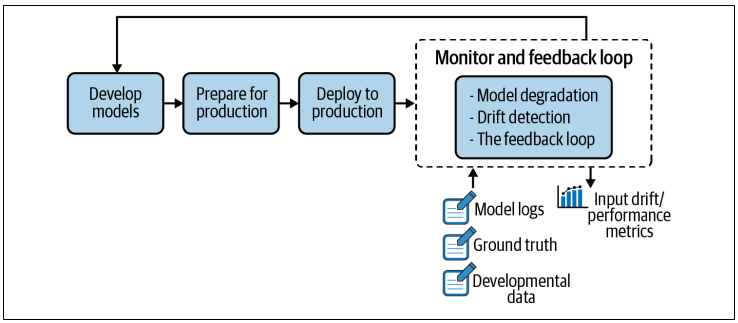
\includegraphics[scale=0.5]{images/monitor-intro}
    \label{fig:monitor-intro}
\end{figure}



Understanding Model Degradation
Once a machine learning model is trained and deployed in production, there are two
approaches to monitor its performance degradation: ground truth evaluation and
input drift detection. Understanding the theory behind and limitations of these
approaches is critical to determining the best strategy.\cite{treveil2020introducing}(p.89)

\begin{figure}[!htbp]
    \caption{Continuous delivery for end-to-end machine learning process\cite{treveil2020introducing}(p.95)}
    \centering
    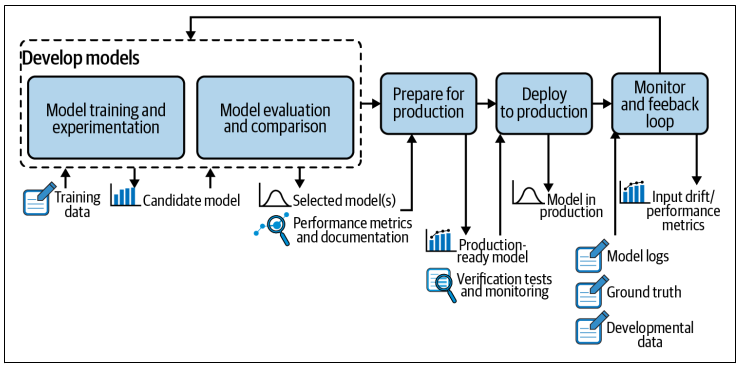
\includegraphics[scale=0.5]{images/feedback-loop-intro}
    \label{fig:feedback-loop-intro}
\end{figure}


As explained in\cite{treveil2020introducing}(p.103), Traditional software is designed to meet fixed specifications and maintains its functionality after deployment.
In contrast, ML models are defined by their statistical performance on specific data, making them prone to performance degradation as data properties change.
Beyond typical software maintenance, ML systems require careful monitoring of performance drift,
with ground truth-based evaluation being essential and drift detection serving as an early warning.
Retraining on new data is the primary solution, though model adjustments are also possible.
Improved models can be validated using shadow scoring or A/B testing to ensure enhanced performance before deployment.

The frequency of model retraining depends on factors like the domain, the cost of retraining, and the potential performance improvement.
Teams must balance these considerations, such as whether the retraining cost justifies the performance gain or if sufficient new data is available to enhance the model.\cite{treveil2020introducing}(p.86)

\subsection{Architecture, infrastructure and existing platforms}\label{subsec:architecture-infrastructure-and-existing-platforms}
Figure\ref{fig:infra} shows a reference architecture proposed by\cite{10855428} based on their results.
Their proposed solution integrates GitHub Actions, Docker, and Kubernetes for the DevOps component, complemented by a robust ecosystem of tools:
Feast for metadata storage, Mlflow as the model repository, Kubeflow for model orchestration, and Flower for distributed computing.
This combination creates a comprehensive and scalable MLOps framework.

\begin{figure}[!htbp]
    \caption{MLOps reference architecture\cite{10855428}}
    \centering
    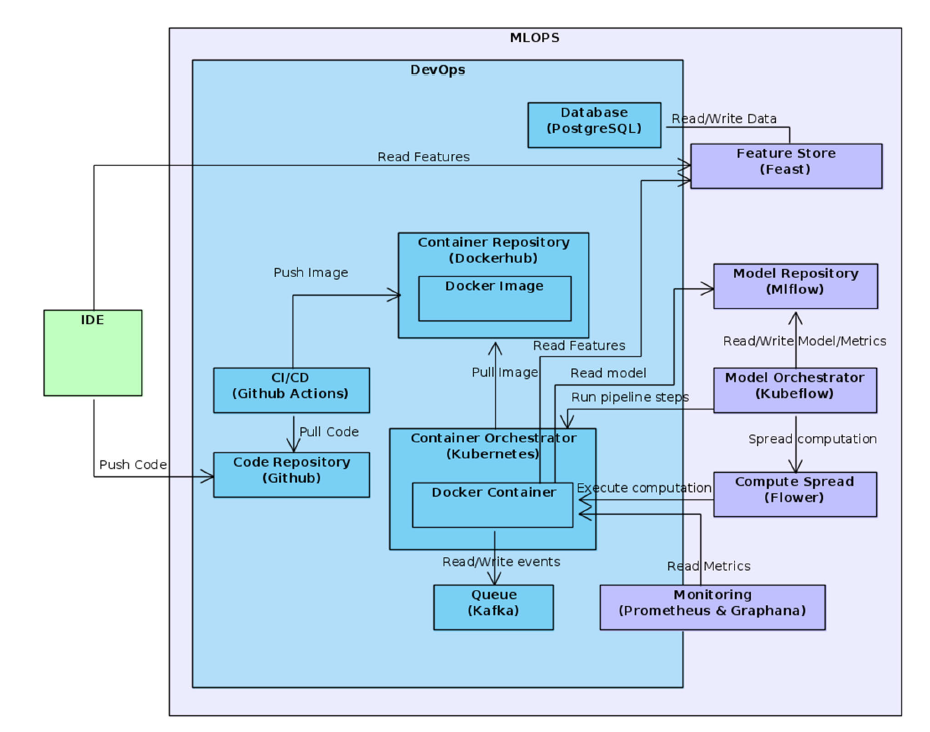
\includegraphics[scale=0.5]{images/infrastructure}
    \label{fig:infra}
\end{figure}


The Acumos AI platform\cite{10690392} is an open-source project that propose a platform that allows to hotswap models and deploy
them to wellknown cloud providers (targets like Kubernetes, AWS, Azure or GCP).
By using microservices, they made it easier to swap the models hidden behind a REST API\@.

The Nifi project\cite{10346079} uses the Acumos project to demonstrate how to take an ML model
to production.
The Nifi project implement automatic and reusable ML model training and ML model serving pipelines.

Reusable MLOps is still a novel concept\cite{10690392}.

The OCDL platform\cite{LIU2020704} was built on Kubernetes and other open-source frameworks to provide a scalable solution.
It also integrates with GitHub to enable CI/CD pipelines and delivery, as illustrated in Figure\ref{fig:ocdl}.
OCDL provides an online IDE for model coding, a reusable code template, data access and GPU/CPU computing instances\cite{LIU2020704} .

\begin{figure}[!htbp]
    \caption{The OCDL architecture layers\cite{LIU2020704}}
    \centering
    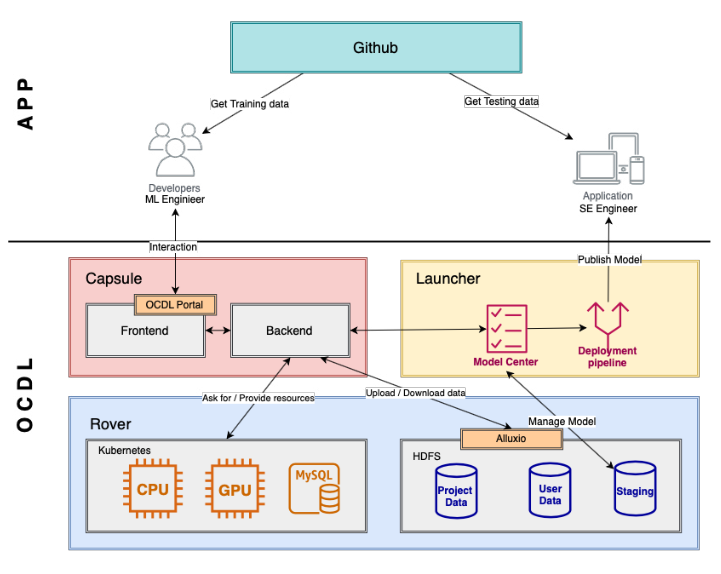
\includegraphics[scale=0.5]{images/ocdl-architecture}
    \label{fig:ocdl}
\end{figure}

We will use all their remarks and experiment to create our own.

The more complete proposition of an architecture and workflows was found was in\cite{Kreuzberger2022MachineLO}.
It will be an inspiration to implement our workflow and can be found in fig\ref{fig:end-to-end-workflow}

\begin{figure}[!htbp]
    \caption{MLOps Architecture proposed in \cite{Kreuzberger2022MachineLO}}
    \centering
    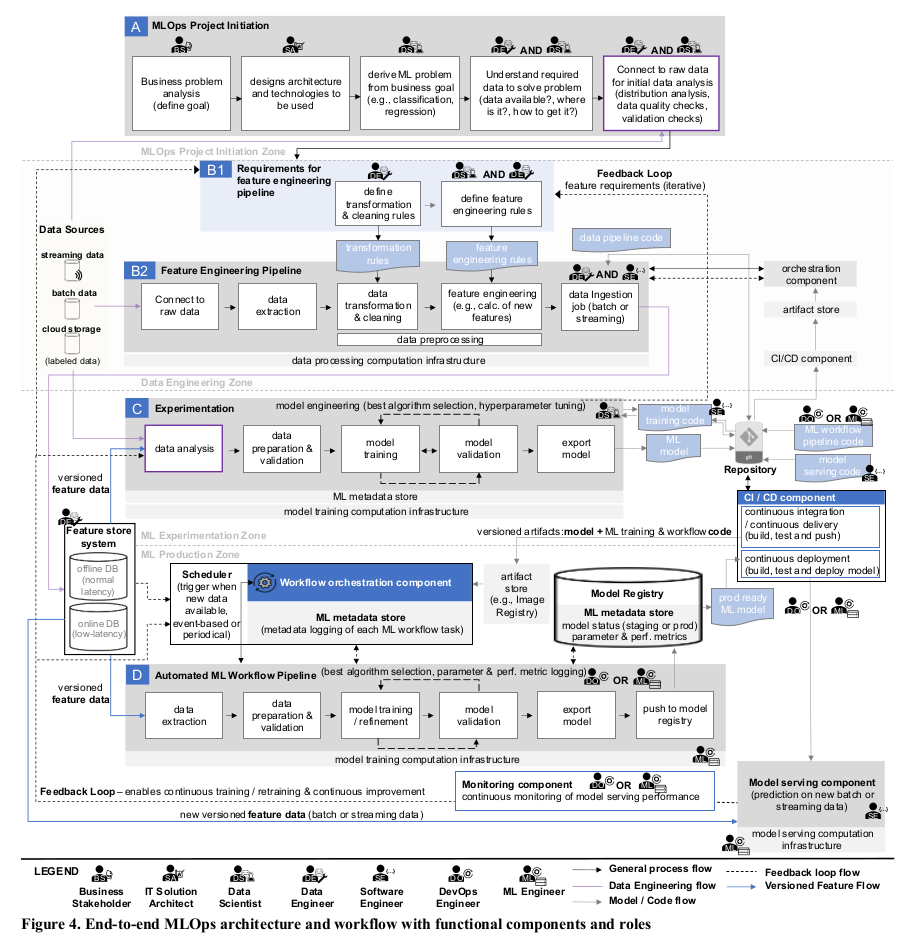
\includegraphics[scale=0.5]{images/kreuz-end-to-end-workflow}
    \label{fig:end-to-end-workflow}
\end{figure}

\subsection{Maturity Models}\label{subsec:matutiry-models}
The authors of\cite{mlops-maturity-model}, they propose a maturity model that goes from manual MLOps to fully automated MLOps.
It differs from the Microsoft and the Google MLOps maturity models,
but they all tend to go from manual to fully automated MLOps processes using automated CI/CD and
ML pipelines.\cite{mlops-definition-tools-and-challenge}

In their research\cite{inproceedings} also identifies key motivators for MLOps and proposes three levels of MLOps maturity.
Level 3 being the most sophisticated and recommended for enterprise solutions.

\begin{figure}[!htbp]
    \caption{Maturity levels \cite{mlops-maturity-model}}
    \centering
    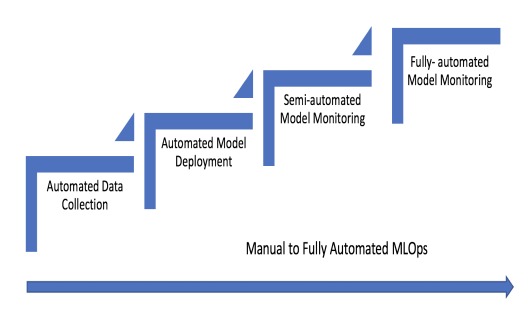
\includegraphics[scale=0.5]{images/maturity-levels}
    \label{fig:maturity}
\end{figure}

\subsubsection{AutoML}

AutoML automates the machine learning process, including tasks like data preparation, model creation, hyperparameter tuning, and evaluation,
making it simpler and more accessible.
It is increasingly integrated into MLOps platforms, enabling companies to deploy ML models into production more efficiently.
Major cloud platforms now offer AutoML tools, enhancing productivity and feasibility for cloud-based ML projects.
This combination of AutoML and MLOps is driving broader adoption across industries.\cite{gift2021practical,mlops-definition-tools-and-challenge}
